\documentclass[11pt,a4paper]{article}
\usepackage{tabularx}
\usepackage{ltablex}
\usepackage{graphicx}
\usepackage[cache=false]{minted}
\setminted[erlang]{
frame=lines,
framesep=2mm,
baselinestretch=1.1,
fontsize=\footnotesize,
linenos,
breaklines}
\setminted[haskell]{
frame=lines,
framesep=2mm,
baselinestretch=1.1,
fontsize=\footnotesize,
linenos,
breaklines}
\setminted[bnf]{
frame=lines,
framesep=2mm,
baselinestretch=1.1,
fontsize=\footnotesize,
linenos,
breaklines}
\usemintedstyle{friendly}
% Add Subtitle
\usepackage{titling}
\newcommand{\subtitle}[1]{%
  \posttitle{%
    \par\end{center}
    \begin{center}\large#1\end{center}
    \vskip0.5em}%
}

\begin{document}

\title{Advanced Programming}
\subtitle{Exam 2018}

\author{Exam Number: 95, Username: zlp432}
\date{\today}
	
\maketitle
\tableofcontents

\section{Utility functions}
The Code for this task is attached in the appendix \ref{appendix:question1-1}.

\subsection{Version}
The Implementation of Version is relatively straight forward and throughly tested by unit tests, which include the examples from the exam text.
I did ended up with a not working implementation before, so I ended up reimplementing the function which is now working as it should.

\subsection{Merge}
Merge is implemented as described in the exam text and tested with many different examples in the unit tests, which all run through.
I had some problems with matching the constraints together, since I kind of lost overview of the function.
Especially ending up when merging only with same package and the different ones (not matching) where not added to the resulting list but in the end just forgot to append the rest to the result.

\subsection{Assessment}
The Utility functions seems to work as intended, as least I was able to reuse them in the parser, and thanks to lots of unit tests to both functions I do believe they work as they should.

\section{Parsing appm databases}
\subsection{Choice of parser library}
I implemented the Parser for appm in parsec, mostly out of this reason:
\begin{itemize}
	\item Better Error handling compared to ReadP
	\item I do have more experience with Parsec then ReadP (Assignments)
\end{itemize}

I did end up using \textbf{try} quite a lot, which wasn't my intention at all but with the presented Grammar I haven't found a better solution and overall the parser works more or less.

\subsection{Grammar}
I decided to make a more strict choice about the Clauses, by parsing them in a fixed ordering (name first etc.), I didn't find much of a better solution for that grammar.



\subsection{Assessment}
I did quite a few unit tests for the parser (including failing ones), since not everything ended up to be working or there was just not enough time left to fixing all the bugs which showed up.
%\subsection{Transform Grammar}
%The existing grammar has some ambiguities, like allowing many names, version etc. which now transformed to only allow once
%\begin{minted}{bnf}
%Database ::= \epsilon

%\end{minted}

\section{Solver}

\section{Earls of Ravnica}
The code for this task can be found in Appendix
\subsection{Solution}
\subsection{Implementation}
The earls of Ravnica can be seen as a state machine for which I chose to use gen\_statem.
The following states exist:
\begin{itemize}
	\item Under Configuration
	\item Under Activation
	\item Active
	\item Shutting down
\end{itemize}

\begin{figure}[!htb]
	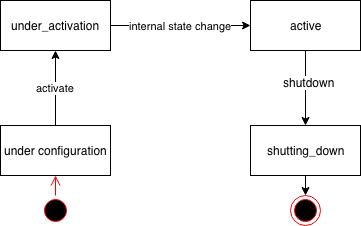
\includegraphics{images/ravnica}
	\caption{Simple State machine diagramm}
\end{figure}

\subsection{Data Structure}
The Data structure I used to implement Ravnica consists of a map with following entries:
\begin{itemize}
	\item \textbf{description} Saves the description which gets saved when starting a server
	\item \textbf{connections} Map for Handling the connections from one District to an other
	\item \textbf{creatures} Map for handling all the entered/active creatures on a Server
	\item \textbf{trigger} Set a trigger for a district
\end{itemize}

\subsection{All states}
Messages which get accepted in all states.
\subsubsection{get\_description}
Gets the description \texttt{Desc} which gets set on create of a District.

\subsection{Under configuration}
As soon as a Server started it is in the under\_configuration state.
\subsubsection{connect}
Connects 2 District with a Action, by saving it in the \texttt{connections} map, 
connects can only be made while district is under configuration in other states an error gets returned.

\subsubsection{trigger}
Under configuration also a trigger can be added to the server, here always the last one gets taken (overwritting whit the newest one).
Trigger gets rung whenever a creature enters or leaves a district.

\subsection{Under activation}
When \texttt{activate} gets called the district and it's neighbors need to get activated, under\_activation is a intermediate state until all neighbors and the district itself are activated.
In case the neighbors can't be activated (for example when a neighbor got shutdown), then the server goes back to the state of under\_configuration.

\subsubsection{activate}
Activate tries to activate all it's neighbors and changes the state of the server to \texttt{active} or back to \texttt{under\_configuration}.

\subsection{Active}
In the active state, no more new connections can be added, also no triggers.
So as soon as a district and it's neighbors is activated, it should only be possible to either run \texttt{get\_description}, \texttt{enter} or \texttt{take\_action} and of course shutting down.

\subsection{Shutting down}
When shutting down is called all neighbors of a district will be shut down as well and this can be propagated until all districts and it's nieghbors are shutdown.

\subsubsection{shutdown}

\subsection{Territories with cycle}

%\section{Solution}
%\subsection{Files}
%\subsection{Running the programm}
%\subsection{Running the tests}
%\section{Implementation}
%\subsection{Gen-Statem}

%\subsection{Data Structure}
%\subsection{All states}

%\section{Assessment}

%\subsection{Scope of Test Cases}

%\subsection{Correctness}

%\subsection{Code Quality}

\appendix
\section{Code Listing}
\subsection{Question 1.1: handin/appm/src/Utils.hs}
\label{appendix:question1-1}
\inputminted{haskell}{handin/appm/src/Utils.hs}
\subsection{Question 2.1: handin/ravnica/district.erl}
\inputminted{erlang}{handin/ravnica/district.erl}
%\inputminted{erlang}{handin/src/quizmaster_helpers.erl}

\end{document}